\documentclass[../main.tex]{subfiles}
\graphicspath{{\subfix{../images/}}}
\begin{document}

  A seguir, serão apresentados os resultados preliminares e os experimentos realizados com o Caramelo. 
  
  \subsection{Testes preliminares}
  
  Os resultados preliminares referem-se aos resultados obtidos com as funcionalidades básicas do robô: capacidade de movimentação a partir do modelo cinemático e capacidade de controle da orientação do corpo com o controlador de angulação.

  Primeiramente, foi avaliada a movimentação do corpo a partir do modelo cinemático. Foi observado que o sistema não só é capaz de realizar a cinemática de cada uma das pernas individualmente como também do seu corpo em todos os 6 graus de liberdade (translações em $x$, $y$ e $z$ e rotações em $roll$, $pitch$ e $yaw$). A figura \ref{fig:moving_body} ilustra o movimento do corpo do robô em cada um desses graus de liberdade.

  \begin{figure}[!htb]
    \centering
    \caption{Movimentação do corpo do robô.}
    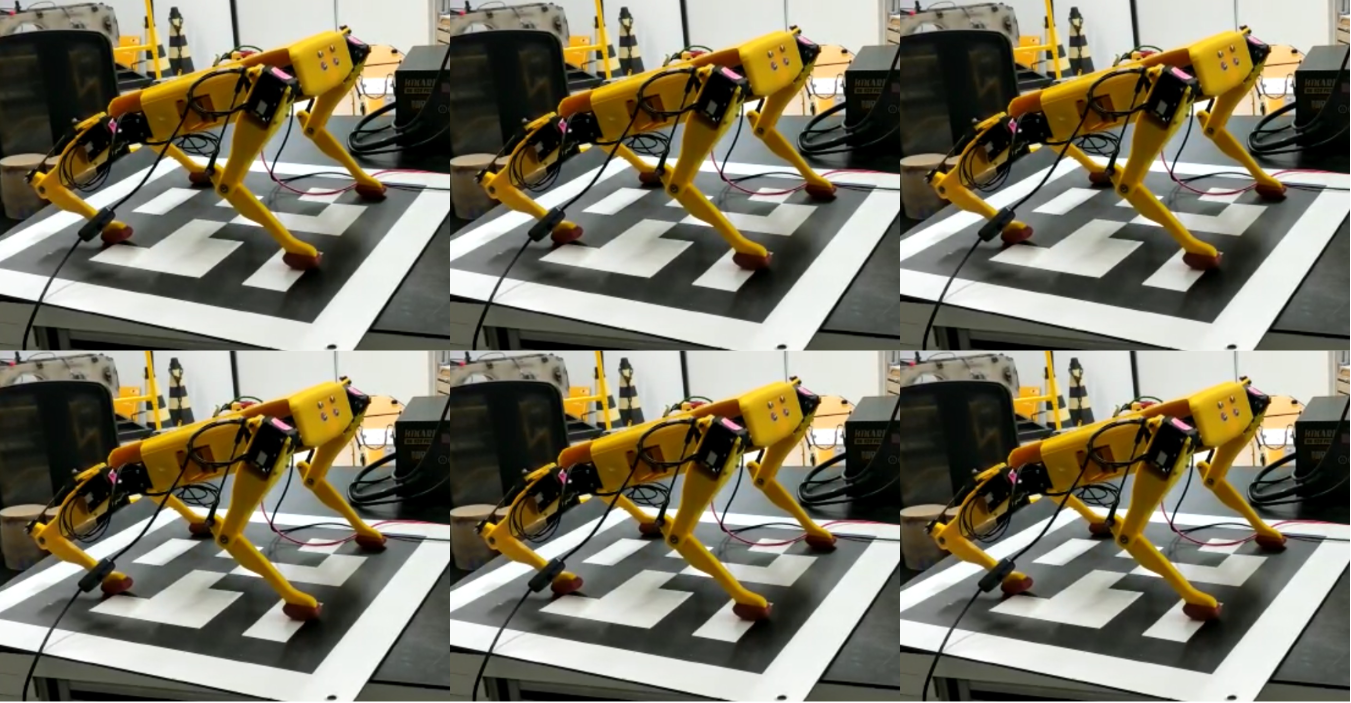
\includegraphics[width=0.48\textwidth]{moving_body.png}
    Fonte: autores.
    \label{fig:moving_body}
  \end{figure}

  A seguir, foi avaliada a performance do controlador de angulação do corpo. Os gráficos da figura \ref{fig:grafico_controlling} ilustram o comportamento do sistema à variação dos \textit{setpoints} de orientação em \textit{roll} e em \textit{pitch} para o corpo do robô ao longo do tempo. As curvas em azul representam os \textit{setpoints} aplicados como sinais degrau, enquanto que as curvas em vermelho ilustram o comportamento do sistema. 

  \begin{figure}[!h]
    \centering
    \caption{Respostas dos controles de angulação.}
    \begin{subfigure}[t]{0.48\textwidth}
      \centering
      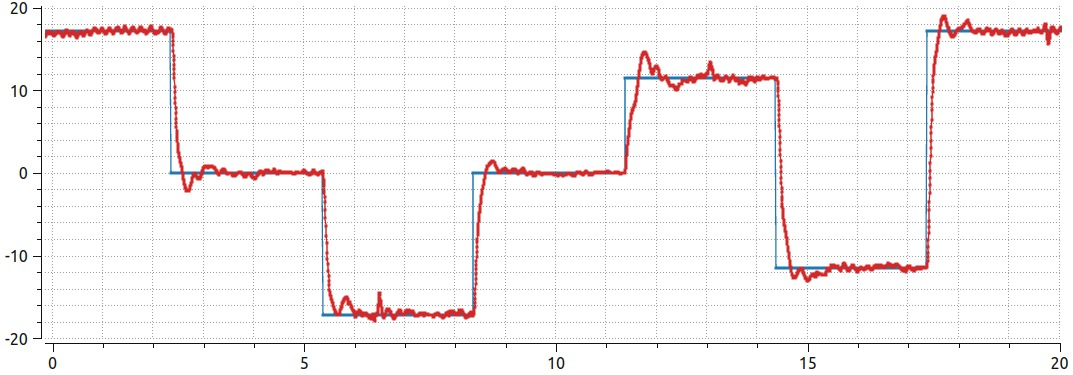
\includegraphics[width=1.0\textwidth]{grafico_controlling_X.png}
      \caption{\textit{Roll.}}
      \label{fig:controlling_roll}
    \end{subfigure}
    \begin{subfigure}[t]{0.48\textwidth}
      \centering
      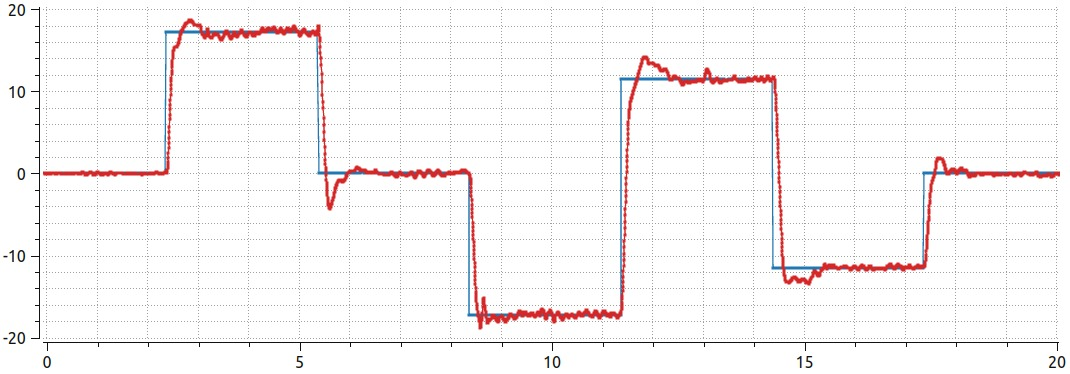
\includegraphics[width=1.0\textwidth]{grafico_controlling_Y.png}
      \caption{\textit{Pitch.}}
      \label{fig:controlling_pitch}
    \end{subfigure}
    Fonte: autores.
    \label{fig:grafico_controlling}
  \end{figure}

  Nota-se que o protótipo é capaz de se adaptar rapidamente aos novos valores desejados de orientação simultaneamente em ambos os eixos.

  \subsection{Experimentos}
  A seguir, serão apresentados os resultados dos experimentos descritos na seção \ref{sec:method_results_analysis}.

  \subsubsection{Análise de trajetória}
  \label{sec:trajectory_analysis}
  O objetivo desse experimento foi analisar o tempo de execução da trajetória, as coordenadas finais $(x_{final}, y_{final})$ da pata e a altura máxima $z_{max}$ atingida durante o passo, comparando-os com os valores esperados para cada um desses parâmetros. A tabela \ref{tab:trajetoria} mostra as médias e desvios padrões encontradas para cada um desses parâmetros durante a realização do experimento.

  \begin{table}[!htb]
    \caption{Resultados do experimento da trajetória da pata.}
    \centering
    \begin{tabular}{ccc}
      \hline
      \textbf{Teste} & \textbf{1}      & \textbf{2}  \\
      \hline
      $\bar{tempo} (s)$         & 0,557  & 0,557 \\
      \hline
      $\sigma_{tempo} (s)$       & 0,008  & 0,008 \\
      \hline
      $\bar{x}_{final} (cm)$     & 5,034  & 3,024 \\
      \hline
      $\sigma_{x_{final}} (cm)$  & 0,009  & 0,013 \\
      \hline
      $\bar{y}_{final} (cm)$     & 2,924  & 4,915 \\      
      \hline
      $\sigma_{y_{final}} (cm)$  & 0,013  & 0,004 \\      
      \hline
      $\bar{z}_{max} (cm)$       & 4,760  & 4,755 \\      
      \hline
      $\sigma_{z_{max}} (cm)$    & 0,023  & 0,028 \\
      \hline   
    \end{tabular}

    Fonte: autores.
    \label{tab:trajetoria}
  \end{table}

  Inicialmente, foram removidos os \textit{outliers} (valores do conjunto de dados acima ou abaixo dos limites superior e inferior, respectivamente) das amostras, valores que fogem da normalidade e podem prejudicar a análise dos dados. Em seguida, a fim de avaliar a normalidade dos dados, foram aplicados testes de Shapiro-Wilk nos dados de tempo e altura máxima de ambos os testes, os quais obtiveram $p_{valor} > 0,05$ em todos os casos. Isso indica que as amostras de ambos os testes estão semelhantes a uma distribuição normal para um nível de confiança de $95\%$. Posteriormente, foram realizados dois testes de análise de variância (ANOVA) unilaterais: o primeiro relacionando o tempo de execução da trajetória nos testes 1 e 2 e o segundo a altura máxima alcançada. O objetivo foi verificar se os resultados se alteraram para diferentes valores de $(x, y)$ requisitados. O resultado da ANOVA indica um $p_{valor}$ de aproximadamente $0,7212$ referente ao tempo e de $0,5070$ referente à altura máxima alcançada durante o passo. Ambos os valores são superiores a $0,05$, indicando que não há uma diferença significativa entre as médias de cada teste, considerando um nível de confiança de $95\%$. Ou seja, diferentes pontos de destino em $(x, y)$ não interferiram no tempo de execução do passo nem na altura máxima alcançada pela pata.

  O gráfico da figura \ref{fig:grafico_trajetoria_xyz} representa uma das amostras coletada para o primeiro teste ($x=0,05m$, $y=0,03m$), correspondente à trajetória em $z$ (altura do passo). Nota-se que, como esperado pela análise da tabela \ref{tab:trajetoria}, há um atraso na execução da trajetória (neste caso específico de aproximadamente $54ms$) e a altura máxima alcançada é levemente inferior à desejada (alcançando neste caso um valor próximo a $0,0476m$).
  
  \begin{figure}[!htb]
    \centering
    \caption{Trajetórias realizadas pelas patas.}
    % 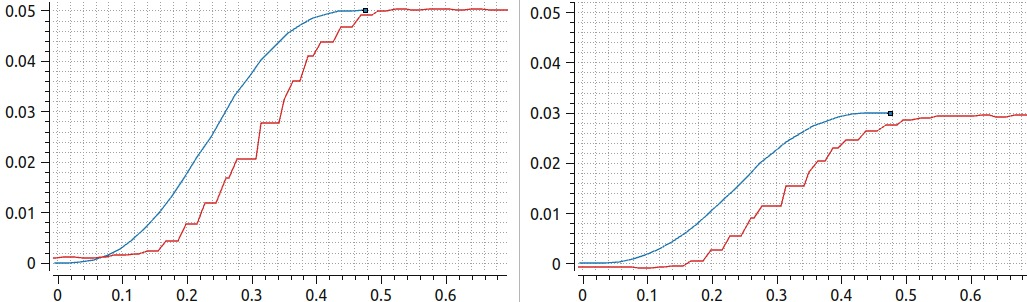
\includegraphics[width=0.48\textwidth]{grafico_trajetoria_xy.png}
    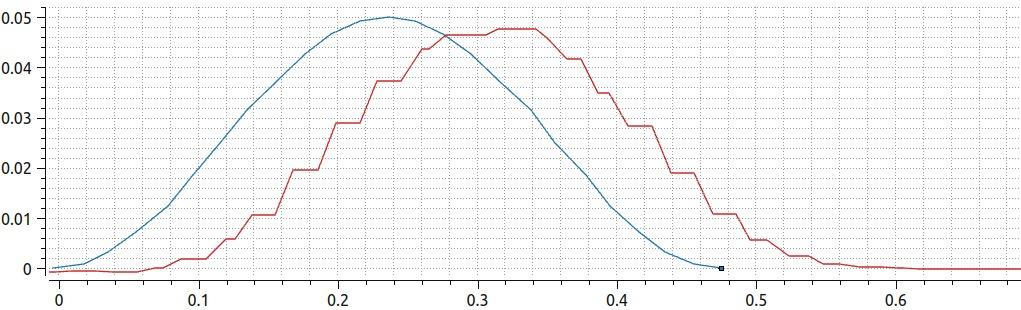
\includegraphics[width=0.48\textwidth]{grafico_trajetoria_z.png}
    Fonte: autores.
    \label{fig:grafico_trajetoria_xyz}
  \end{figure}

  A distribuição das amostras de tempo e de altura máxima da pata em ambos os testes pode ser percebida pelos gráficos de \textit{box plot}, apresentados na figura \ref{fig:time_zmax_traj}. Nestes gráficos, é observado a proximidade entre as medianas dos testes e a similaridade na distribuição dos seus quartis,(representados pelos retângulos). Ainda que haja uma pequena diferença entre os valores mínimos e máximos das amostras, é possível enfatizar a semelhança entre os resultados dos testes 1 e 2.

  \begin{figure}[!htb]
    \centering
    \caption{Tempo e altura da pata durante um passo.}
    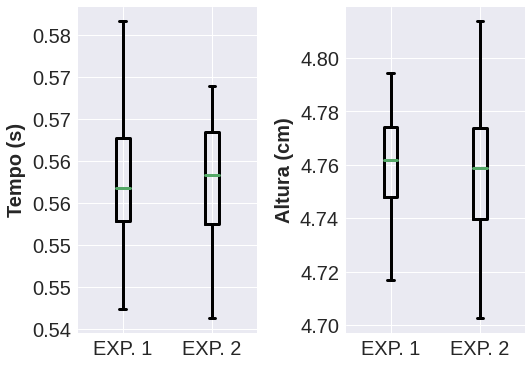
\includegraphics[width=0.48\textwidth]{tempo_zmax_traj.png}
    Fonte: autores.
    \label{fig:time_zmax_traj}
  \end{figure}

  \begin{figure}[!htb]
    \centering
    \caption{Oscilação do corpo em ambos os tipos de terreno.}
    \begin{subfigure}[t]{0.49\textwidth}
      \centering
      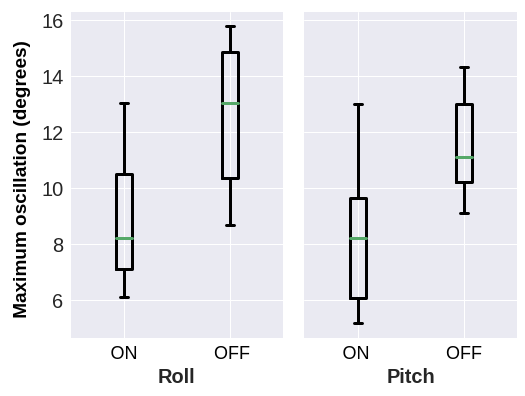
\includegraphics[width=1.0\textwidth]{plane_boxplot.png}
      \caption{Terreno plano.}
      \label{fig:imu_test_plane}
    \end{subfigure}
    \begin{subfigure}[t]{0.49\textwidth}
      \centering
      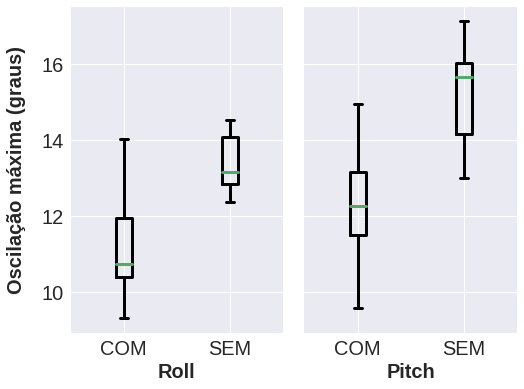
\includegraphics[width=1.0\textwidth]{irregular_boxplot.png}
      \caption{Terreno irregular.}
      \label{fig:imu_test_irregular}
    \end{subfigure}
    
    Fonte: autores.
    \label{fig:imu_test}
  \end{figure}

  \subsubsection{Análise da velocidade e estabilidade}
  Esse experimento teve como objetivo avaliar se o robô consegue se mover em uma velocidade desejada e o quão estável ele se mantém durante a caminhada. Foram coletados dados de velocidade média do robô (inferida com base no tempo que o robô levou para percorrer $1,5m$) e oscilação máxima do corpo em \textit{roll} e \textit{pitch}. As médias e desvios padrões de cada variável para cada teste estão apresentadas na tabela \ref{tab:vel_stab}. 
  
  \begin{table}[!htb]
    \caption{Resultados da análise da velocidade e estabilidade.}
    \centering
    \begin{tabular}{ccccc}
      \hline
      \textbf{Teste} & \textbf{1} & \textbf{2} & \textbf{3} & \textbf{4} \\ \hline
      Ter. & Reg. & Reg. & Irreg. & Irreg. \\ \hline
      \begin{tabular}[c]{@{}c@{}}C. R.\end{tabular} & Não & Sim & Não & Sim \\ \hline
      \begin{tabular}[c]{@{}c@{}}Vel. \\ (cm/s) \end{tabular} &   2,15   &  3,68  &   2,03  & 2,39  \\ \hline
      \begin{tabular}[c]{@{}c@{}} $\sigma_{Vel}$  \\ (cm/s) \end{tabular} & 0,040 & 0,075 & 0,016 & 0,047 \\ \hline
      \begin{tabular}[c]{@{}c@{}} $\Delta_{Roll}$ \end{tabular} & 12,59\degree & 8,81\degree & 13,37\degree & 11,13\degree \\\hline
      \begin{tabular}[c]{@{}c@{}} $\sigma_{Roll}$ \end{tabular}  & 2,54\degree & 2,36\degree & 0,78\degree & 1,47\degree \\ \hline
      \begin{tabular}[c]{@{}c@{}} $\Delta_{Pitch}$ \end{tabular} & 11,55\degree & 8,31\degree & 15,19\degree & 12,09\degree \\ \hline
      \begin{tabular}[c]{@{}c@{}} $\sigma_{Pitch}$ \end{tabular}  & 1,89\degree & 2,63\degree & 1,44\degree & 1,66\degree \\ \hline

    \end{tabular}
    Fonte: autores.
    \label{tab:vel_stab}
  \end{table}

  A partir desses dados, foi observado que o robô não alcançou a velocidade desejada de $0,05 m/s$ em nenhum dos testes, alcançando apenas $74\%$ desse valor para a média de velocidades do teste feito em terreno plano com controle de estabilidade ativo. É possível justificar essa diferença pelo acúmulo de erros nas coordenadas finais $(x_f, y_f)$ das patas a cada passo nesse cenário em que os atuadores do robô operam com carga. Isto é, ao operar sustentando o peso do robô, o sistema de controle não foi capaz de seguir fielmente a trajetória do passo, percorrendo com a pata uma distância menor do que a necessária para alcançar uma velocidade média de $0,05 m/s$. Esse resultado é diferente do que foi mostrado na seção \ref{sec:trajectory_analysis}, onde os motores foram avaliados em um cenário sem carga significativa.
  
  A tabela \ref{tab:vel_stab} também mostra que as oscilações médias em \textit{roll} e \textit{pitch} foram menores quando o controle de estabilidade estava ativo tanto no terreno plano quanto no irregular. A fim de comprovar que o controle de estabilidade contribuiu efetivamente para diminuir as oscilações do robô em ambos os tipos de terreno, o mesmo procedimento de análise do experimento anterior foi seguido. Primeiramente, foram removidos os \textit{outliers} das amostras e aplicado o teste de normalidade de Shapiro-Wilk, o qual indicou um $p_{valor} > 0,05$ para todos os casos. Em seguida, foi aplicado o teste ANOVA para comparar a oscilação em \textit{roll} e em \textit{pitch} dos testes 1 e 2. O mesmo processo foi repetido para os testes 3 e 4. O resultado da análise apontou que as distribuições de oscilação em \textit{roll} e \textit{pitch} são significativamente diferentes tanto no terreno plano quanto no terreno irregular, uma vez que o $p_{valor}$ de todos os testes foi inferior a $0,05$. Os gráficos da figura \ref{fig:imu_test} ilustram com mais detalhes a distribuição dos dados. Nota-se que com o controle de estabilidade, a oscilação foi mais dispersa na maioria dos testes, o que pode ser comprovado analisando os desvios padrões apresentados na tabela \ref{tab:vel_stab}. No entanto, exceto para a oscilação em \textit{roll} no terreno plano, o terceiro quartil está abaixo do primeiro quartil das distribuições de oscilação sem o controle de estabilidade, mostrando que o controlador diminuiu a oscilação do corpo do robô em \textit{roll} ou em \textit{pitch} em pelo menos $75\%$ das amostras coletadas.

  % \subsection{Testes complementares}
  % Como resultados complementares, foi observado que o robô possui a habilidade de andar por terrenos inclinados. Durante o teste, o robô foi capaz de se locomover por um plano inclinado com aproximadamente 5,3$\degree$ de inclinação (figura \ref{fig:tests3-4}). 

  % O último teste constatou que o robô é capaz de ultrapassar pequenos obstáculos. Para isso, foram considerados degraus de três diferentes alturas: 2, 4 e 5 $cm$ (figura \ref{fig:tests3-4}). O robô foi capaz de superar degraus de 2 e 4 $cm$, porém falhou ao tentar subir um de 5 $cm$.

  % \begin{figure}[!htb]
  %   \centering
  %   \caption{Fotos do robô no teste da rampa e do degrau.}
  %   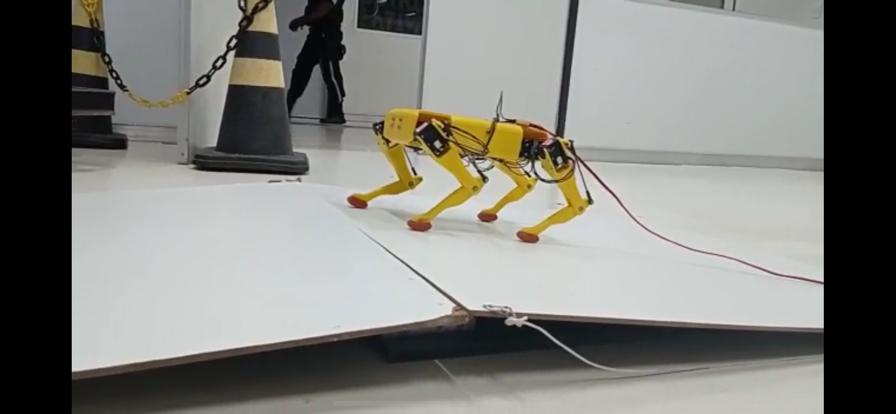
\includegraphics[width=0.48\textwidth]{ramp_test.jpeg}
  %   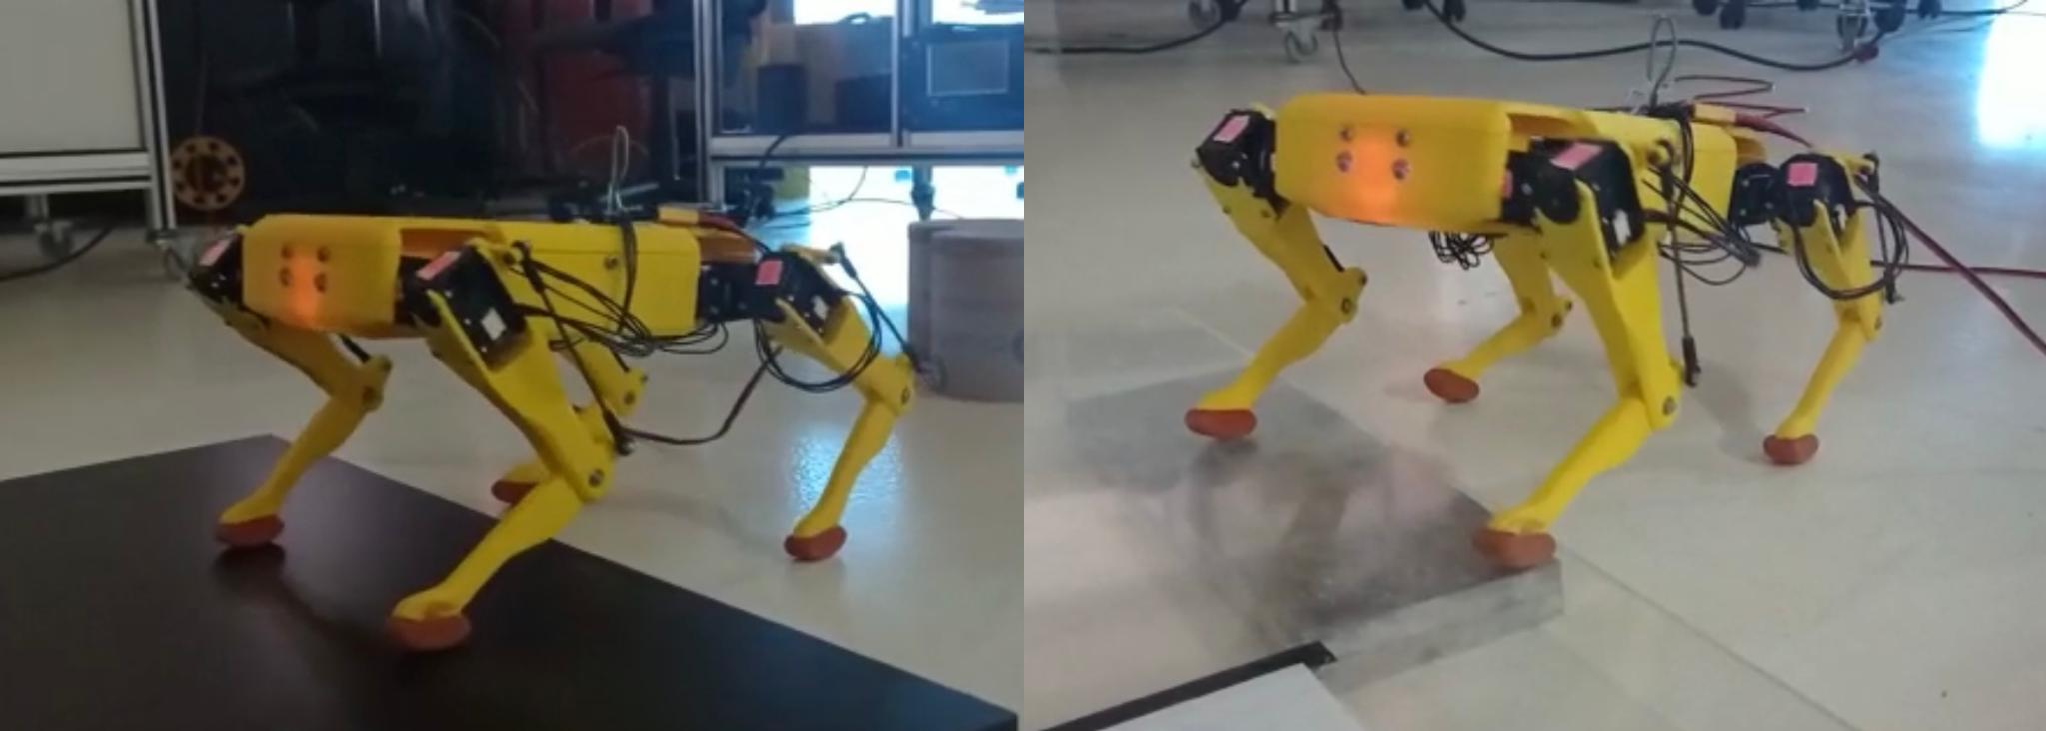
\includegraphics[width=0.48\textwidth]{test4.png}

  %   Fonte: autores
  %   \label{fig:tests3-4}
  % \end{figure}

\end{document}